% Paper for Learning-Based Controls (ME 537)

\documentclass[letterpaper, 10 pt, conference]{ieeeconf}  % Comment this line out if you need a4paper

\IEEEoverridecommandlockouts                              % This command is only needed if 
                                                          % you want to use the \thanks command

\overrideIEEEmargins                                      % Needed to meet printer requirements.

\usepackage{prg-stuff}

%\usepackage{ijcai09}  % style
\usepackage{times}    % font
\usepackage{graphicx} % inserting images
\usepackage{cite}
%\usepackage{amsmath}
\usepackage{mathtools} % For math
\usepackage{hyperref}
%\usepackage{enumitem}
\renewcommand{\deg}{\ensuremath{^{\circ}}\xspace}  % why doesn't this work???

\providecommand{\e}[1]{\ensuremath{\times 10^{#1}}}

\graphicspath{ {./figures/} } % Point to the figures directory

%%%%%%%%%%%%%%%%%%%%%%%%%%%%%%%%%%%%%%%%%%%%%%%%%%%%%%%%%%%%%%%%%%%%%%%%%%%

\title{\LARGE \bf 
O Rover Where Art Thou?\\
Multi-Robot Exploration with Limited Sensor Capabilities
}

\author{Kory Kraft$^{1}$, Austin Nicolai$^{2}$, and Matthew Rueben$^{3}$% <-this % stops a space
%\thanks{*This work was supported by... }% <-this % stops a space
\thanks{*All authors are with the School of Mechanical, Industrial, and Manufacturing Engineering,
         Oregon State University,
         Corvallis, OR, USA. }% <-this % stops a space
\thanks{$^{1}$Corresponding author: {\tt\small kraftko@onid.oregonstate.edu}}%
\thanks{$^{2}$Corresponding author: {\tt\small nicolaia@onid.oregonstate.edu}}%
\thanks{$^{3}$Corresponding author: {\tt\small ruebenm@onid.oregonstate.edu}}%
}

\begin{document}

\maketitle
\thispagestyle{empty}
\pagestyle{empty}

\begin{abstract}
Sensor input plays a vital role in robotics.
We analyze the impact of 3 important sensor characteristics: sensor range,
field-of-view, and sensor noise utilizing 3 common reward structures in the 
exploration domain. Domain triviality in relation to sensor settings is discussed.
Our important contributions are twofold: we show that the 
difference reward is robust to sensor changes, whereas 
the local reward structure, in our domain, is susceptible to sensor variation.
We also created a novel construct, the POI sensitivity gradient, that allows
quick mapping and visualization of the regions in the world which
contain the most useful sensor information.  
\end{abstract}


\section{Introduction}
The decreasing costs and increasing capabilities of computer hardware and software make
robots an increasingly attractive alternative to human labor. More specifically, robots have 
been targeted for use in the exploration domain, both in single agent and 
multi-agent systems.  Robots have the potential to
handle certain extreme environments better than their human
counterparts.  They can cover large swaths of territory more
efficiently, or conversely fit in very tight spaces without disturbing
the surrounding environment (e.g. snake robots). 

A number of inroads have been made into harnessing the power and
advantages of robots in the exploration domain. NASA continues to use
the rover Curiosity to explore Mars. Several companies have built
mobile robots to explore and decontaminate the the Fukushima Daiichi
nuclear power station after the 2011 meltdown \cite{nuclear_robots}. Added to these
accomplishments, robots are increasingly being used with other robots, 
adding significance to multi-agent systems (MAS) studies.

Previous MAS research, however, often fails to fully consider the effect of
sensor limitations upon the learning algorithm within given domains. In many realistic cases, sensors fall drastically short of being able to see the entire search space at once. Many lower-cost robots are now using the Microsoft Kinect because it offers RGB-D sensing for fewer than 100 dollars. Albeit, the Kinect is constrained by a 0.8 - 4.0m distance range and 57$^{\circ}$ horizontal and 43$^{\circ}$ vertical field-of-view. On top of all this, there is ever present sensor noise; a constant source of frustration for sensor precision and accuracy.

As always, decreasing hardware costs do not mean infinite hardware resources.
Implementers must be able to make informed decisions on the cost-benefit tradeoff 
between fewer, higher-performing sensors and additional lower-performing sensors. Moreover, cost-benefit analysis needs to be done on a level that includes sensor impact on  agent performance within a given domain. Specifically, we will show the trade-offs between using varying quality sensors and the overall system performance by modeling robots with different sensor ranges, fields-of-view, and noise characteristics in the rover domain utilizing three common reward structures. Our analysis necessitated some preliminary work that forms a second major contribution; namely, the creation of a novel construct, the POI sensitivity gradient, that allows
quick mapping and vizualisation of the regions of the world which
contain the most useful sensor input.  Our work will help future implementers conduct more accurate cost-benefit analyses in order to make wiser decisions when building and deploying robots in the real world.


\section{Related Work}
\subsection{Exploration Domain}
In the exploration domain, agents must discover all areas of an
initially unknown map. One method tackles the search of complicated
areas via cellular decomposition and systematic coverage \cite{choset2001coverage}. Another
method examines the effect of limited knowledge on an agent. It
examines how well different algorithms utilize agents, as well as how
the number of rooms and room size effects the explorability of a space
\cite{ferranti2007brick}. Lastly, one method coordinates exhaustive exploration of a space
by intelligently assigning destinations to different agents \cite{burgard2005coordinated}.

\subsection{Credit Assignment}
An important and particulary difficult aspect of MAS is the problem of
credit assignment. Agent to agent coordination involves individual
agents working together on a common task or goal. Since one agent’s
behaviors might affect other agents, however, the learning process
becomes hard. Chalkiadakis and Boutilier \cite{chalkiadakis2003coordination} develop a way to weigh
the costs and benefits of taking non-greedy actions during
reinforcement learning based on the value of the new information that
might be gained. They also give the agents some limited ability to
reason about how their actions influence others. Another question is,
what does each agent know about the other agents? This is the
information by which they can coordinate at all. Gmytrasiewicz and
Durfee \cite{gmytrasiewicz2000rational} expand the typical state space of each agent by adding
knowledge about other agents’ knowledge, which is recursive by
nature. They develop a framework whereby this representation is
usable, however, and present their findings as a move towards
coordinated robot actions. Finally, Burgard et al. \cite{burgard2005coordinated} address
coordination in an exploration scenario, which for them boils down to
intelligently placing goal locations (or waypoints, by extension) for
each agent.

\subsection{Reward Structure}
The structural credit assignment problem is defined as the difficulty that arises in properly assigning credit to a specific agent in a pool of agents.  While this problem has been extensively studied, three overarching reward structures have been developed: the full system reward, the local reward, and the difference reward (\hspace{1sp}\cite{weiss2013multiagent}).  The full system reward, also known as the global reward, assigns the full system reward to each agent in the system.  The local reward assigns a reward to each agent using only information local to the agent. The difference reward is calculated directly or approximated for each agent by artifically removing the agent from a system and replacing the agent's action(s) with another action (which may or may not be legal within the system) and comparing it with the global reward when the agent was in the system. The difference reward is both factored and learnable by definition. It has also been shown to be a superior reward structure in domains where it is computationally tractable. To our knowledge, there has not been extensive research demonstrating the advantages or disadvantages of each of these reward structures in the face of various sensor limitations (e.g. \cite{tumer2002learning, turner2006designing}). 

\subsection{Sensor Limitations}
A limited sensor range can cause two potential problems for agents:
collision with each other and sub-optimal behavior due to lack of
coordination. Dimarogonas et al. \cite{dimarogonas2007decentralized} and Do \cite{do2007bounded} present planning approaches to collision avoidance with limited sensor range. To plan agent motion, both approaches use potential fields (also called
navigation functions) that include some potential or proximity function between each pair of agents that can see each other. The ant colony problem presented by Gordon et al. \cite{gordon2004gathering} examines the case where the sensors have limited range and no distance information, i.e., only output the direction to sensed entities. All of these approaches involve sending the agents to some goal location or formation, not exploring an area, and no machine learning techniques are used. One approach that used reinforcement learning examined reward-shaping in a noisy domain involving competitive robotic “foraging”. It was shown that intelligent reward-shaping and algorithms were able to overcome the noise present and achieve good performance \cite{mataric1997reinforcement}.

\subsection{Noise}
Noisy sensors are a reality for robots. Lower-cost sensors, like the Microsoft Kinect, have the potential to significantly drive down costs for using robots for exploration. However, lower-cost sensors also bring with them higher noise characteristics. Specifically the Microsoft Kinect has been shown to have a random error in the depth axis ranging from a few mm to 4 cm in a non-uniform distribution \cite{khoshelham2012accuracy,nguyen2012modeling}. Techniques have been developed to overcome the various types of sensor noise, both by modifying sensor output and modifying learning techniques, but these still leave sensor information imperfect \cite{nguyen2012modeling,hu2010distributed}. Before spending more time and resources trying to overcome the complications that arise due to sensor noise by adding or improving hardware or software, it is important to understand how sensor noise actually impacts rover performance within a given domain.


\section{Methods}
\subsection{Domain}
This work is a direct extension of that described by Tumer and Agogino
(2008, \cite{agogino2008analyzing}). Therein, the goal of the rovers is to observe the more
important points of interest (POIs) at close range in order to earn a
large overall system reward. We use the static POI domain, meaning the POI values and locations are chosen randomly at the
beginning of a training session, and then do not vary for the duration of the episode. The POIs are placed randomly using a single random distribution. The sum POI value is 1000, resulting in a maximum system reward of 40.  Each POI is assigned in the following manner: one POI is valued at half of the POI sum value, 500.  The remaining POIs are randomly assigned a value summing up to 500.  This ensures that the domain is non-trivial and that a random-walk is not always optimum.  For each learning episode, the rovers begin in at the same location on the map, each with a random heading. The episode
ends after 15 time steps and rewards are assigned. Each rover can move
continuously in two dimensions, and 10 percent noise is added to the
intended movement to simulate real-world errors.

\subsection{Reward Structure}
The global reward presented by Tumer and Agogino (2008) is based on
the closest observation of each POI by any rover:
  
\[
G= \sum_j  \frac{V_j}{min_i \: \delta(L_j, L_i)}
\]

The distance function is the square of the Euclidean norm up to a
minimum distance \(d^2\):

\[
\delta  (x,y) = max \big\{||x - y||^2, d^2 \big\}    
\]

The local reward is perfectly learnable for each rover because it only accounts for that rover's actions. If we sacrifice a bit of computation speed, we can have a reward structure that is both well-factored and learnable in the difference reward.

\[
P_i=G(z_{-i})
\]
\[
D_i=G(z)-G(z_{-i})
\]

\subsection{State Information}
Each rover has two types of sensors. The first type returns an
aggregate score that represents the POI values near the
rover:

\[
s_{1,q,i} =  \sum_{J \in I_q}  \frac{V_j}{\delta (L_j, L_i)} 
\]

The second sensor type returns a similar aggregate for other rovers:

\[
s_{2,q,i} =  \sum_{i' \in N_q}  \frac{V_j}{\delta (L_{i'}, L_i)}  
\]

Each rover’s surroundings are divided into four quadrants and two
sensors -- one POI sensor and one rover sensor -- look out on each
quadrant. Eight total sensors therefore yield eight continuous state
variables.

\subsection{Action Selection and Learning}
State information was mapped to action choices using a neural network with
8 inputs, 10 hidden nodes, and 2 outputs. The activation functions
were sigmoidal and each output value was scaled based on a maximum
movement (4 world units) allowance per step (d is maximum movement per time step and
o1, o2 are the perceptron outputs):

\[
dx = 2d(o_1-0.5)
\]
\[
dy = 2d(o_2-0.5)
\]

An evolutionary algorithm was used with simulated annealing to find
neural networks that yielded good performance. This is called “direct
policy search” because we use an evolutionary algorithm to search for
a good policy directly, i.e. we do not maintain state-action value
estimates as in approaches like Q-learning. The neural network was initialized with randomly
valued weights between \(\pm\)0.5.  A pool of 40 neural networks was assigned for each agent.  40 random
teams were then created using a unique agent and a previously unselected neural network associated with that agent.
A fitness was assigned to the neural network following the episode based on the reward structure in use at 
the time.  An epsilon-greedy selection process was used to pick the best half of the neural network performers for each agent.  An 
epsilon-greedy approach was used to switch one of the better performers (excluding the highest performer) with a lower performer in 
order to further exploration.  The neural networks were mutated by adding a random Gaussian noise with a mean of 0 and a standard deviation of .5 to a given weight, for a percentage of all weights that decreased during training time.
The agents were trained for 75 episodes each.

The system described thus far provides the basis for our study of sensor limitations. Our novel
study regarding sensor impact the impact of domain on learning is detailed below.

\subsection{Rover Heading}
The heading of the rovers is important in our implementation because, for some cases described below, we will restrict the sensor fields-of-view. Imagine if each rover only had a single Microsoft Kinect sensor, pointing forward. We want the rovers to be able to control where this sensor is pointing. 

Each rover begins the episode with a random heading between 0$^{\circ}$ and 360$^{\circ}$. This heading is updated at each time step after the rover moves. The new heading points in the same direction as the rover's chosen movement vector. We chose this protocol because it resembles the way a differential-drive robot would turn towards its destination before driving there. 

\subsection{Sensor Evaluation}
Sensor impact upon learning was evaluated by comparing the baseline
system performance from \cite{agogino2008analyzing} with the system performance after limiting
the sensors in three ways: reducing range, adding noise, and reducing
the field-of-view angle.  Following \cite{agogino2008analyzing}, we defined system performance
as the sum global reward achieved.  Noise was defined as the random
error in a rover’s distance measurements. All three types of sensor
limitations were applied to the POI sensors and the rover sensors
equally. Due to the 2D nature of the simulated world, height was
ignored and sensor field-of-view angle was only measured about the
vertical axis.

Each sensor limitation was applied independently at three different
magnitudes for each reward structure.  Thus, 9 sensor tweaks were applied to
the local, global, and difference rewards. The baseline sensor combination was chosen after \cite{agogino2008analyzing} as having unlimited sensor range, zero noise, and a 360° field-of-view. Sensor
range was tested at 2 world units (half the distance the rover can see), 8 world units (twice the distance 
the rover can see), and unlimited world units. Sensor noise was modeled as a unique normal distribution for
each sensed object with standard deviations at 0\%, 10\%, and 30\% of the
object’s true range. Rover viewing angles were tested at 90$^{\circ}$, 270$^{\circ}$,
and 360$^{\circ}$.

Statistical system runs were executed for 75 episodes for each
sensor/reward structure setup for 10 homogeneous agents.  Overall system reward was then plotted for each
sensor attribute and reward structure.


\section{Interactions between Domain and Learned Policy}
\subsection{Controller Sensitivity to State Information}
Very early in our implementation efforts, we saw that the learned policies of the rovers could be described in terms of two aspects:

\begin{enumerate}
\item \emph{Sensitivity or Reactivity.} The neural networks are constructed such that a rover can learn to respond to changes in sensor (state) information by changing its direction (i.e., action). If it learns to do this, then we say that the rover is \emph{sensitive} to changes in its state information, or that it \emph{reacts} strongly to such changes. This behavior is most directly influenced by the neural network weights that mediate the connections between inputs and the single hidden layer. These input weights determine for each input (here, a POI or rover sensor) how much influence, if any, it will have on the action output of the neuro-controller. 

\item \emph{Direction Bias.} If these input weights make the inputs too large or too small, they will leave the range within which the sigmoidal activation functions of the hidden nodes are sensitive (i.e., about -5 to 5). In this case, changes in the input values (i.e., POI and rover sensor information) will cause only negligible changes to the hidden layer outputs, and the weights between the hidden layer and the output nodes will control the system. This causes behavior that is learned, but insensitive to sensor information; for our problem setup, this means a straight-line trajectory. In our domain, the rover can only here learn the angle and speed of that trajectory. Assuming the speed is sufficient to reach the border of the map, the angle becomes very important for ensuring that the rovers spread out to cover all the POIs. 
\end{enumerate}

Sensitivity can be estimated by how much an agent changes direction throughout its trajectory, especially as large sensor changes occur (e.g., passing by a rover or high-valued POI). A comparison of learned rover behavior that is sensitive and insensitive is shown in Figure \ref{fig:sensitivity}. All rovers in that scenario have learned and indeed converged on their demonstrated behavior. 

\begin{figure}[h!]
    \centering
    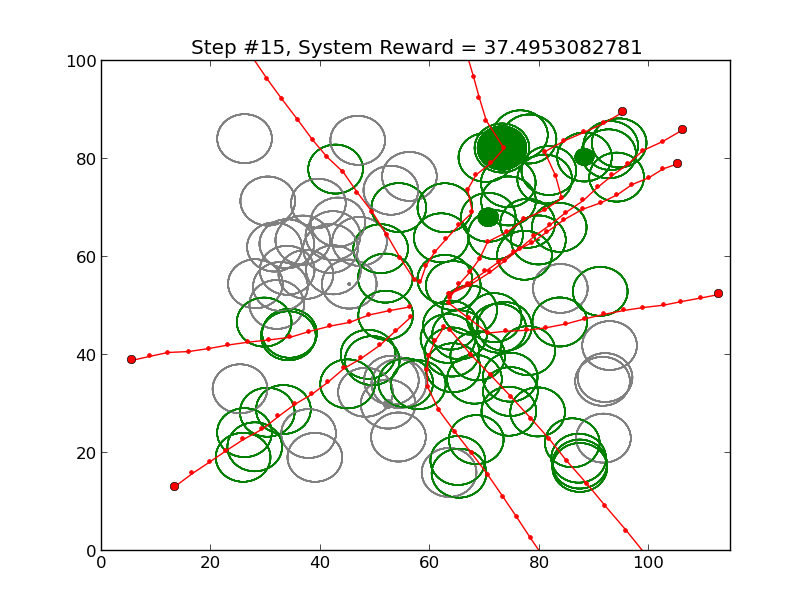
\includegraphics[width=0.45\textwidth]{GlobalMvt75Eps100POIsBaselineSensor.png}
    \caption{Visualization of one episode using a learned rover policy. The reward was global. Two rovers in the bottom-left corner learned straight-line paths that ignore changing sensor information. This is sub-optimal for this domain, as the rover moving most directly left could do better by looping back upwards. In the top-right corner, the unbalanced POI values encouraged learned sensitivity to changing sensor information. This is apparent because the rovers change directions as the episode progresses. The direction changes are effective at observing more POIs more closely. }
    \label{fig:sensitivity}
\end{figure}


\subsection{Easy and Hard Domains}
We will now discuss the extent to which a domain can encourage or discourage learned sensitivity. 

The first consideration is whether sensor information is even necessary for earning the optimal system reward. In other words, can the rovers fully observe every POI by taking well-distributed, straight-line paths? We can calculate this. The critical parameter is the angular separation between paths; if there are enough rovers and a small enough POI region, the space between paths will be so small that no POI could possibly \emph{not} be fully observed (Figure \ref{fig:triviality}). For our domain, the POIs are bounded within a 70x70 square region with a minimum observation distance of 5; for these parameters, 22 or more rovers could obtain the maximum system reward with straight-line paths. This is why, frustrated with poor learning in our original 30-rover domain, we decided to switch to 10 agents for the work described in this paper.

So what domain characteristics \emph{do} encourage the rovers to learn to use their sensors? Our several guidelines are as follows:

\begin{enumerate}
\item \emph{Non-Trivial Domain.} If evenly-spaced, straight-line paths can't optimally observe all the POIs, then rovers will need to learn to serpentine to cover more space or loop back for another pass after an initial charge through the POI region. Since our setup does not include time as an input, serpentine or zigzag behavior is impossible without changing outputs from the POI and rover sensors (see next guideline). A clearer example of this is when the rover learns to turn around if it overshoots the POI region; this requires sensitivity to a sensor reading that means zero POIs are ahead and many POIs are behind. 

\item \emph{Varying Sensor Signals.} The rovers need to experience a wide variety of sensor signals in order to learn how to respond to them. It's possible for a domain to be non-trivial as defined above but still present a rover with unchanging POI sensor signals (rover sensors will depend on agent policies, not the domain, at least directly). For example, a domain with very low minimum POI observation distances might require lots of maneuvering to optimally explore, but a very uniform distribution of these POIs would make sensor signals relatively uniform as well. Placing POIs in clusters or varying their relative values would make the POI sensor signals more sensitive to where the rover is located and to which direction it's facing. 

Two non-trivial domains that demonstrate these principles are shown in Figure \ref{fig:signal-contrast}. We have created a novel construct for domain evaluation that we call the \emph{POI sensitivity gradient}, calculated as follows. At each XY location in a given domain, the POI sensor value is collected from a single sensor at a single heading. The resultant array is the same size as the map. The gradient of this array is taken, and the x- and y-components of the gradient are combined using a root sum of squares. The process is repeated over the full range of headings (360$^{\circ}$, in 5$^{\circ}$ increments), all values are averaged at each location. The resultant metric represents how much the POI sensor will change due to small rover movements at a given location. Values near zero (cf. top pane of Figure \ref{fig:signal-contrast}) indicate that it's difficult to learn behaviors that react to the POI sensors because the input values hardly change in those areas. 

\item \emph{Attending to Sensors leads to Improved Reward.} For learning to occur, these changing sensor signals must be usable by the rover to increase its assigned rewards. This has been done for us with apparent success by the sensor characteristics prescribed in \cite{agogino2008analyzing}.


%\item Moving POIs. If the rovers must perform well for a wide variety of POI positions and not just a static layout, they must vary their actions between episodes, or perhaps even between time steps.  This requires attention to sensor information in order to differentiate between different POI positions. Caveat: in a trivial domain, e.g., with too many rovers for the area to be covered, it doesn't matter how much the POIs move -- sensor information still isn't useful. Here is an example of POI movement that helps teach the rovers to react to sensor information: a single POI is randomly placed at one of the four corners of the map. 
\end{enumerate}

\begin{figure}[h!]
    \centering
    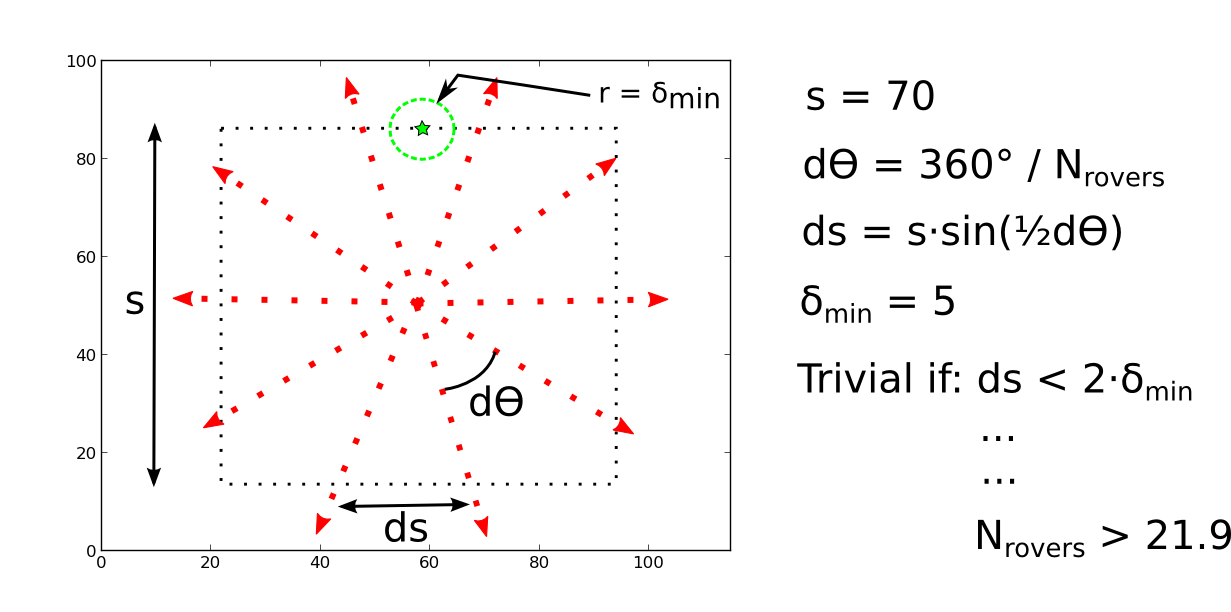
\includegraphics[width=0.45\textwidth]{triviality.png}
    \caption{Definition of a trivial domain for our problem. Rovers are assumed to learn evenly-spaced, straight-line paths. Relevant parameters are the number of rovers, the size of the region containing POIs, and the minimum observation distance for the POIs. In a trivial domain, every POI will necessarily be maximally observed. }
    \label{fig:triviality}
\end{figure}

\begin{figure}[h!]
    \centering
    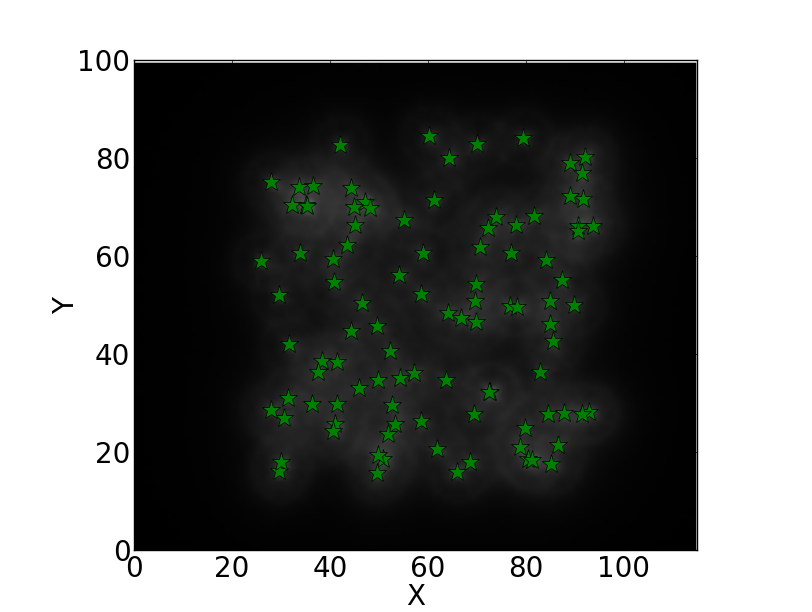
\includegraphics[width=0.45\textwidth]{sensitivity-spread-0.png}
    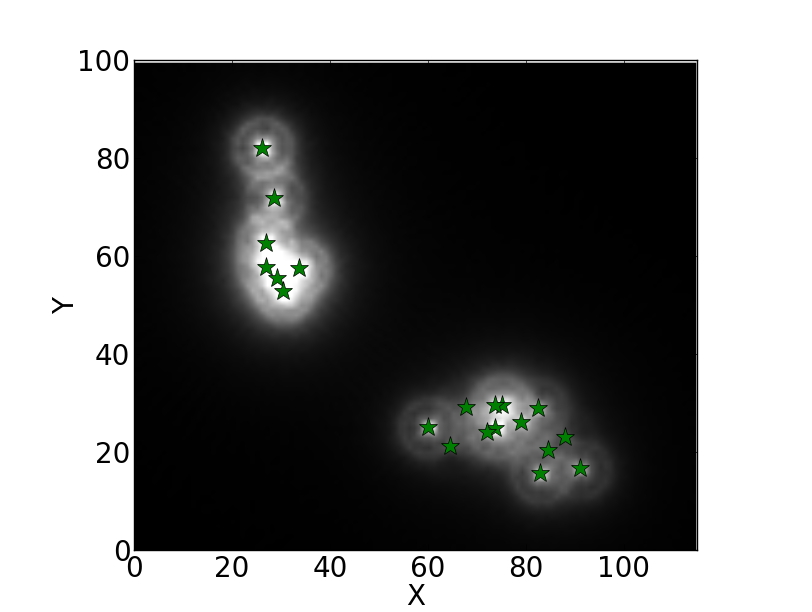
\includegraphics[width=0.45\textwidth]{sensitivity-clustered-1.png}
    \caption{Examples of POI distributions with different POI sensitivity gradients. The POI sensitivity gradient captures the extent to which rover movement would cause POI sensor output changes at a given location. TOP: a uniform distribution of equally-valued POIs yields a low POI sensitivity gradient. BOTTOM: A clustered distribution of weighted-value POIs yields a much higher gradient, but only near the clusters. }
    \label{fig:signal-contrast}
\end{figure}

\section{Results}
\subsection{Reward Structure Comparison}
Before considering any of the sensor limitations, it is important to consider a baseline. Figure \ref{fig:baseline} provides a comparison between the different reward structures considered in this paper. From this figure, it can be seen that while the difference reward learns faster than the global reward, both converge to essentially the maximum possible system reward of 40. The local reward can be seen to improve at first, but then decreases to significantly lower than both the difference and global rewards. This is because as the agents learn with the local reward, many learn to greedily move towards the high valued POI at the expense of the system reward, resulting in unfactored behavior.

\subsection{Sensor Limitations Comparison}
In comparing the different sensor limitations, several conclusions can be drawn. Figure \ref{fig:sensor-range} below shows the effect of limited sensor range, Figure \ref{fig:sensor-fov} shows the effect of limited fields-of-view, and FIgure \ref{fig:sensor-noise} shows the effect of sensor noise. From these figures, it can be seen that the difference reward is the most resilient to sensor limitations; no matter the sensor limitations imposed, the difference reward learns quickly. In general, the more limited the sensor characteristics, the longer it takes the global reward to converge. Of the reward structures evaluated, the local reward is the most perturbed by the sensor limitations.

Specifically, limiting sensor range most influences the learning curves. Most noticeable is the effect on the local reward. This can be seen in [FIGURE NUM] In general, the lower the sensor range, the sooner and more drastically the performance begins to decrease, . One possible explanation is that the more limited the sensor range is, the more likely the agent (when using the local reward) will find one of the high valued POIs and hover near it. Unless the agent randomly explores in such a way to view new POIs and/or rovers, it will not want to leave its current high-value location.

\begin{figure}[h!]
    \centering
    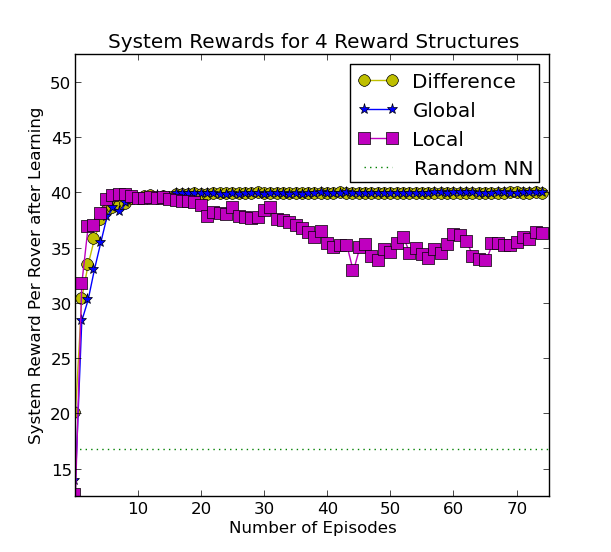
\includegraphics[width=0.45\textwidth]{baseline.png}
    \caption{Comparison of learning curves for three reward structures over 75 episodes. Sensors were unrestricted, i.e., had unlimited sensor range, 360$^{/circ}$ field-of-view, and zero sensor noise. All three curves are compared to the average reward for randomly-initialized, untrained neural networks. }
    \label{fig:baseline}
\end{figure}

\begin{figure*}
    \centering
    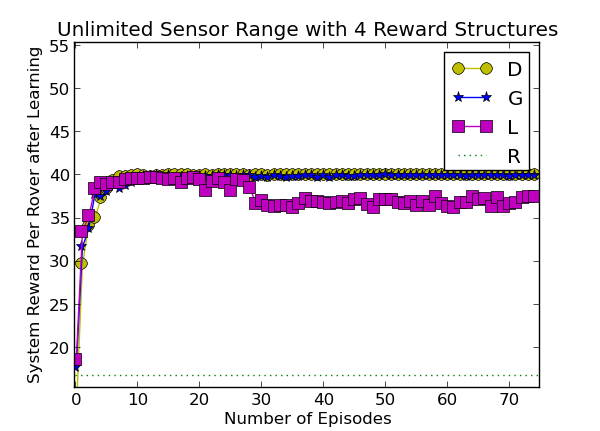
\includegraphics[width=0.3\textwidth]{SR_U.png}
    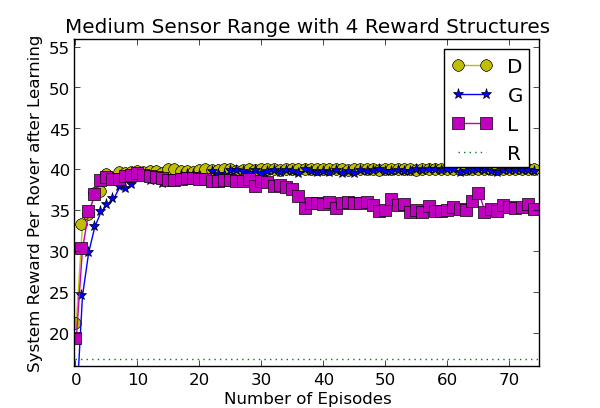
\includegraphics[width=0.3\textwidth]{SR_M.png}
    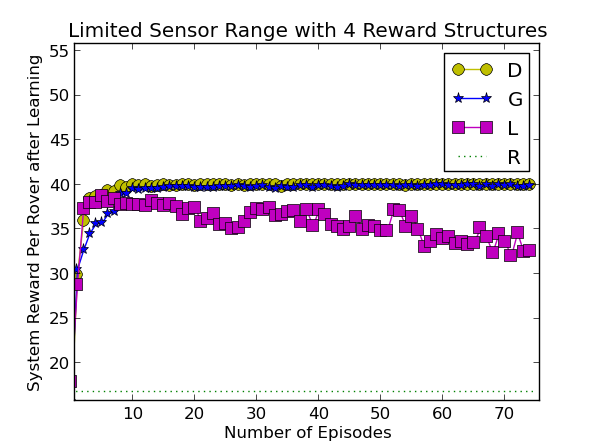
\includegraphics[width=0.3\textwidth]{SR_L.png}
    \caption{Comparison of learning curves for three different sensor ranges over 75 episodes. Sensor ranges were unlimited (left), 8 world units (center) and 2 world units (right). }
    \label{fig:sensor-range}
\end{figure*}

\begin{figure*}
    \centering
    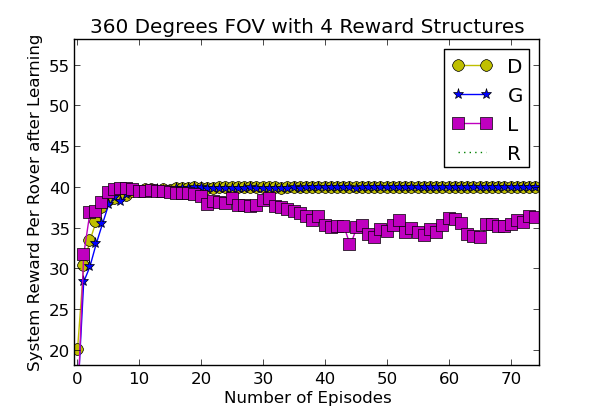
\includegraphics[width=0.3\textwidth]{SF_360.png}
    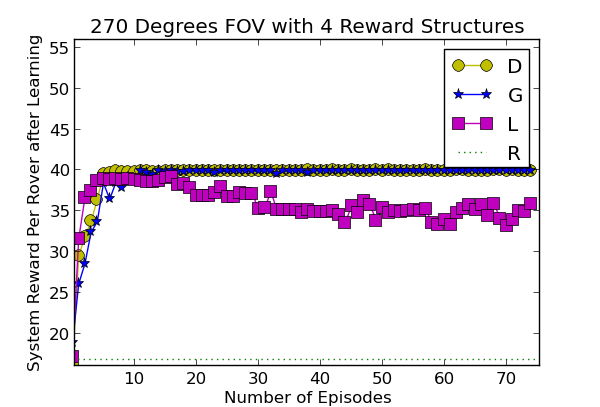
\includegraphics[width=0.3\textwidth]{SF_270.png}
    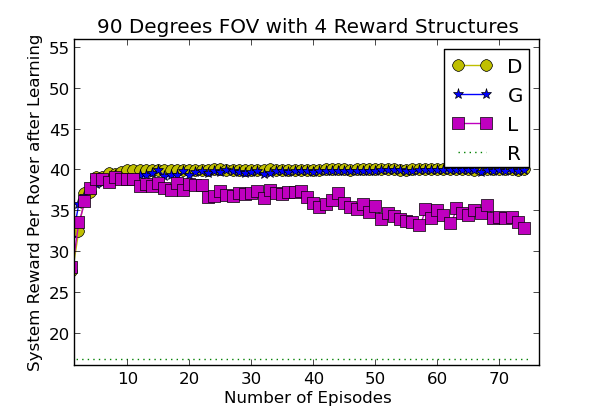
\includegraphics[width=0.3\textwidth]{SF_90.png}
    \caption{Comparison of learning curves for three different sensor fields-of-view over 75 episodes. The chosen fields-of-view were 360$^{/circ}$ (left), 270$^{/circ}$ (center) and 90$^{/circ}$ (right). }
    \label{fig:sensor-fov}
\end{figure*}

\begin{figure*}
    \centering
    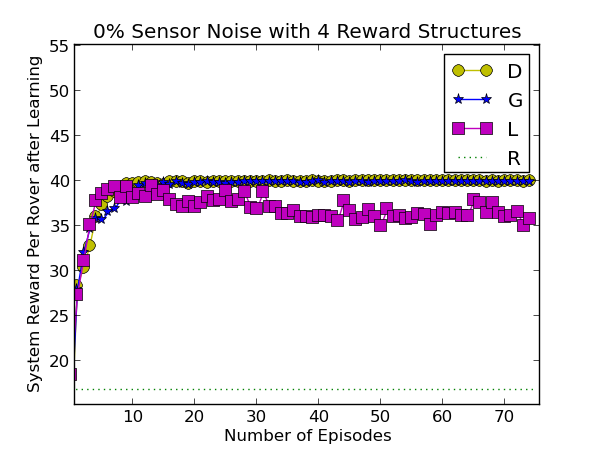
\includegraphics[width=0.3\textwidth]{SN_0.png}
    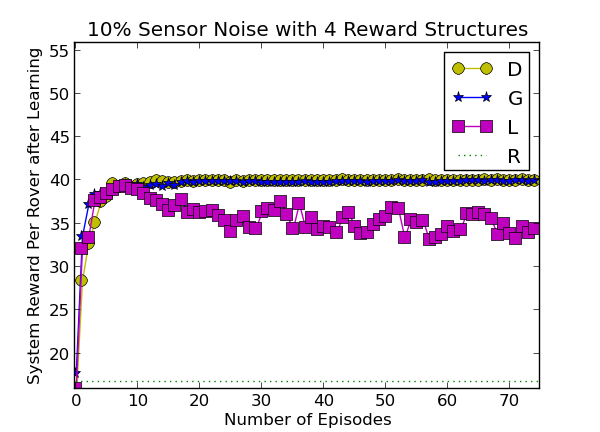
\includegraphics[width=0.3\textwidth]{SN_10.png}
    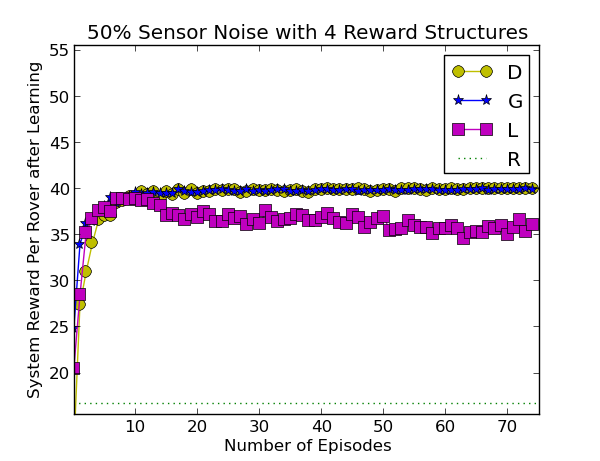
\includegraphics[width=0.3\textwidth]{SN_50.png}
    \caption{Comparison of learning curves for three different sensor noise magnitudes over 75 episodes. The chosen noise levels were 0\% (left), 10\% (center) and 50\% (right). }
    \label{fig:sensor-noise}
\end{figure*}

\begin{figure}
    \centering
    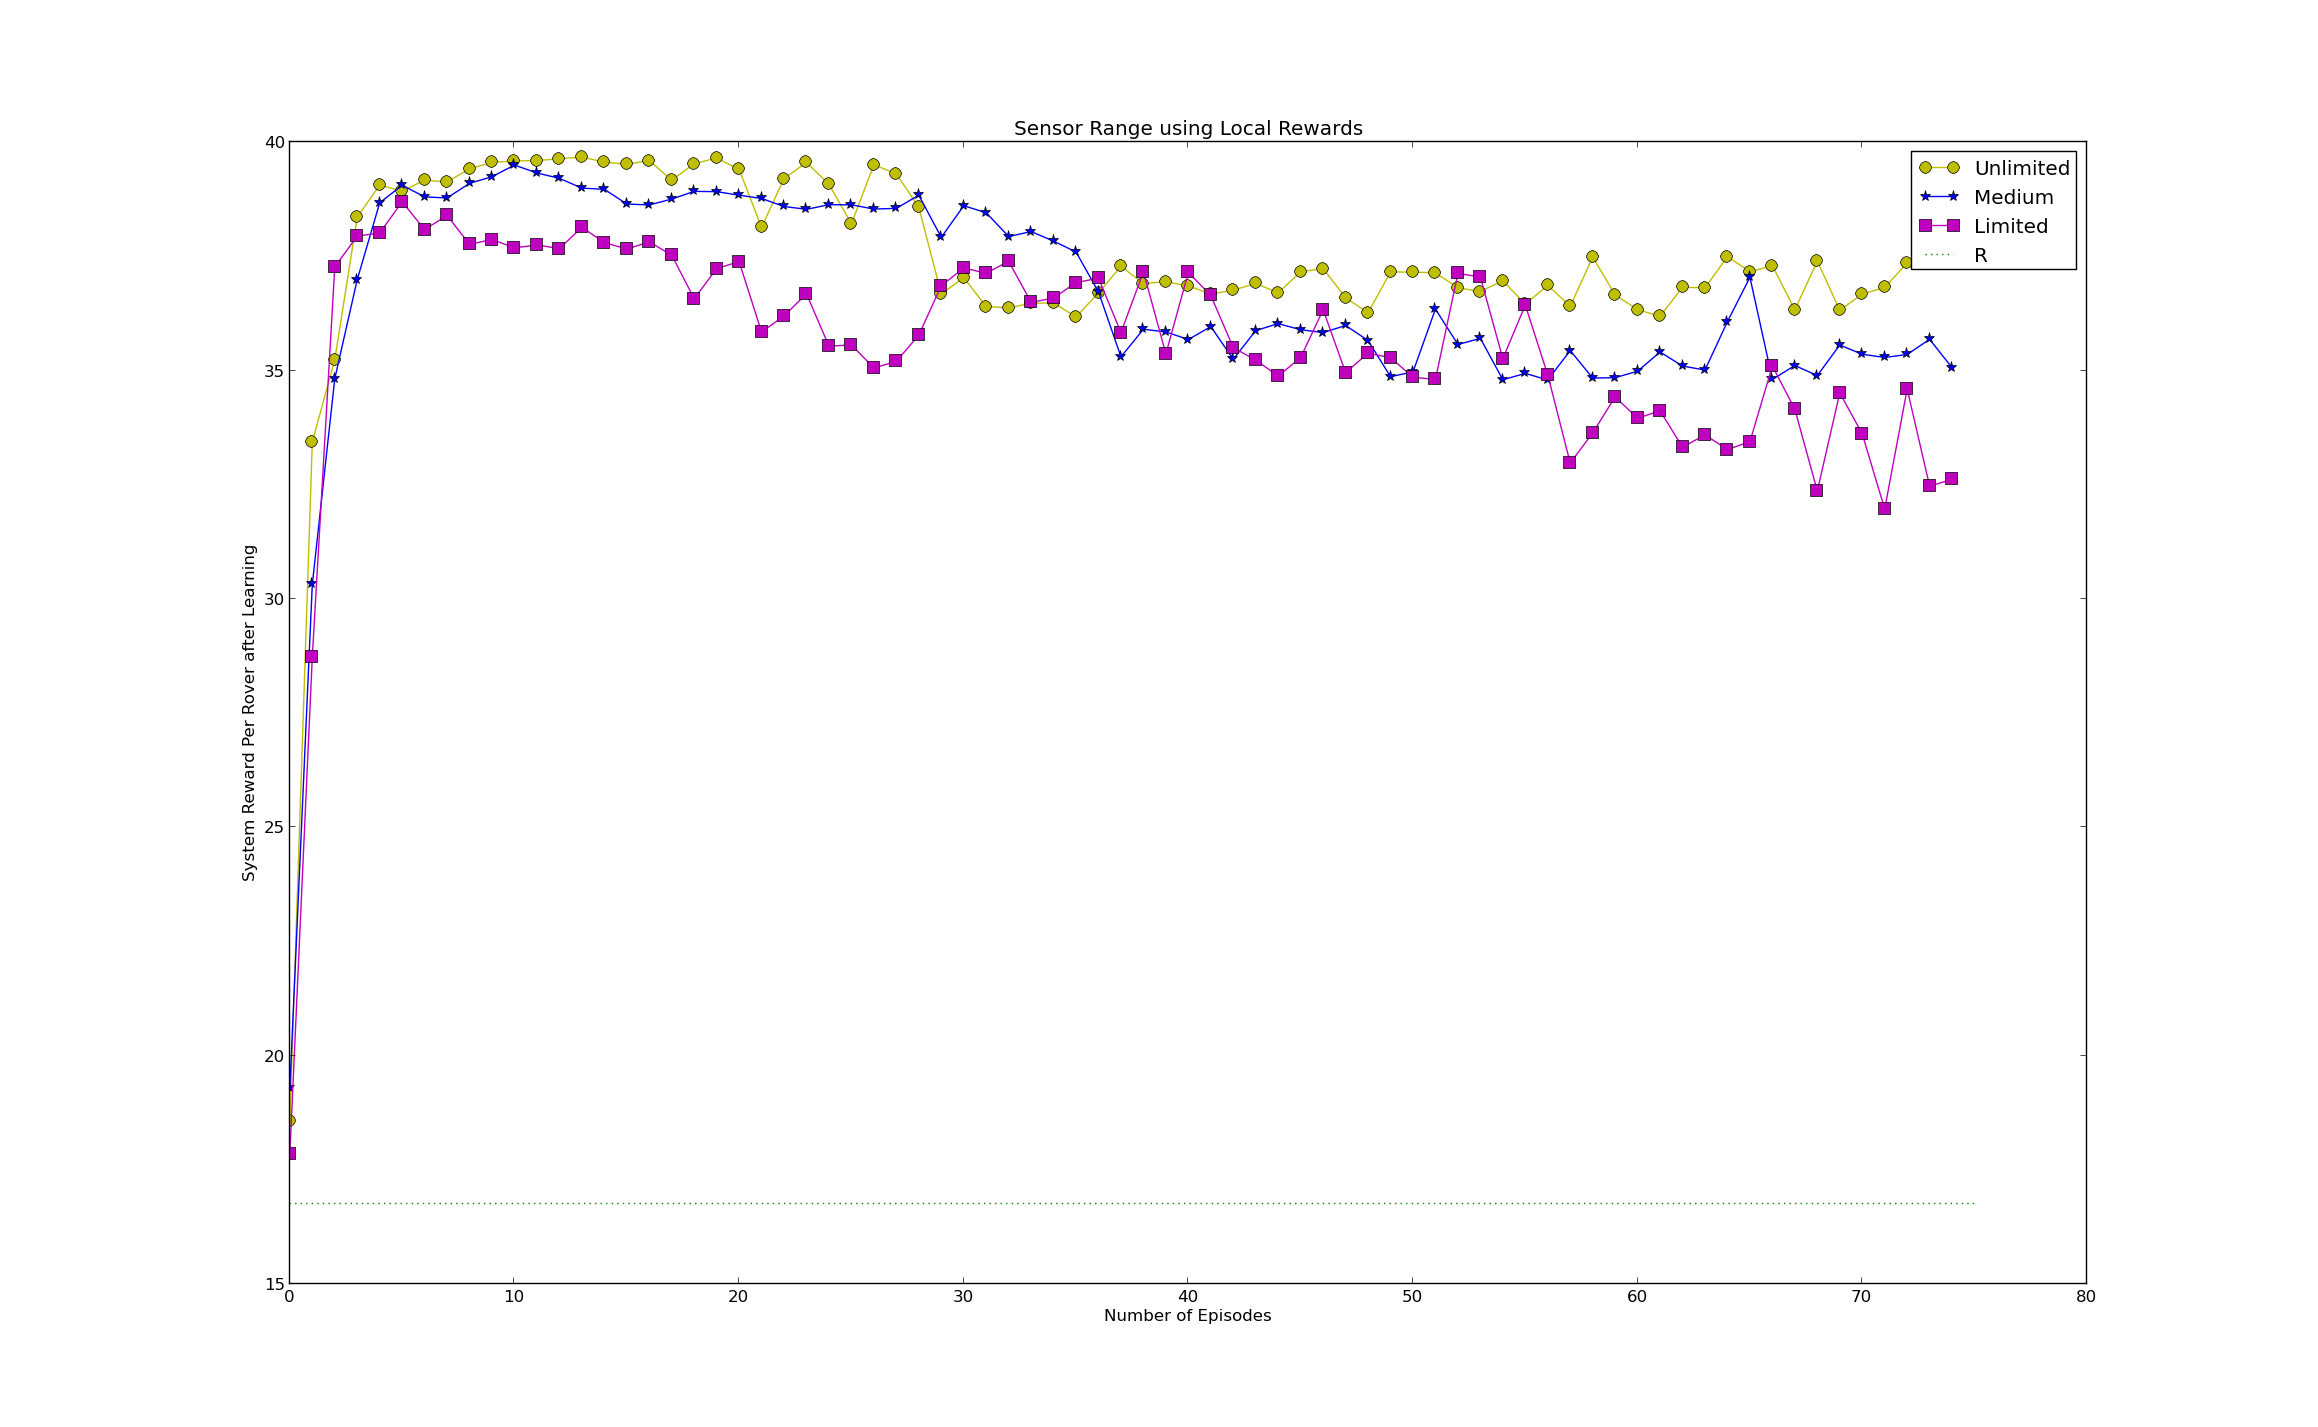
\includegraphics[width=0.45\textwidth]{SR_LocalReward.png}
    \caption{Direct comparison of learning curves using the local reward only for three different sensor ranges over 75 episodes. Sensor ranges were unlimited, 8 world units, and 2 world units. }
    \label{fig:local-reward-comparison}
\end{figure}

\section{Future Work}
The analysis of both our domain and results presents several avenues for further research.

\subsection{Additional Domain Complexity}
The difficulties presented by our original, trivial, domain yield interesting possibilities for future work. Our analysis suggests that specific domain characteristics may have a large impact in system performance. Engineering more complex domains may allow us to observe interesting trade-offs between sensor characteristics and the system reward. Some possible domain changes may include movement restrictions and vision occlusion (e.g. impassable terrain or a wall). Another possibility would be allowing agents to temporarily increase their sensor capabilities, similar to obtaining a better vantage point from a hill. There may exist domains in which limiting one sensor characteristic impacts performance less than limiting another (e.g. limiting sensor range over field-of-view).

Additionally, changing the reward structure allows us to change the nature of our domain. Presenting the agents with more complex reward structures can influence their cooperation and learned policies. With more complex behavior required of the agents, the performance trade-offs between limited sensor characteristics may become more evident. One possible way to increase the reward structure complexity is to require simultaneous POI observation in order to obtain a reward. Another possibility is to explore the issue of temporal credit assignment. If agents are able to better understand which of their actions most contributed to their reward, they are better able to adjust their policy.

\subsection{Sensor Restriction Combinations}
An additional avenue for future work involves exploring additional sensor characteristic combinations. While our current work only dealt with varying one sensor characteristic at a time, this would more closely model real world sensors. In reality, sensors have physical limitations on all characteristics. This work could allow for performance vs. cost comparisons (e.g. perhaps a \$10 sensor with 90$^{\circ}$ field-of-view and 5m sensing range performs only 5 percent worse than a \$500 sensor with 90$^{\circ}$ field-of-view and 30m sensing range).


\subsection{Heterogeneous Agents}
Exploring the performance of different sensor characteristic combinations naturally leads to the question of how a MAS performs when agents in the system have different sensing capabilities. This is an interesting problem because it allows for the simulation of cost constrained systems (e.g. should agents be equipped with several cheaper, specialized sensors or less powerful, but equivalent sensors) as well as analyzing the impact of agent failure (e.g. sensor malfunctions restricting field-of-view or actuator failures preventing agent movement). The presence of heterogeneous agents leads to many interesting questions including: Can how does system performance change if some agents have diminished capabilities? In particular, at what point does performance begin to drastically diminish? Will agents with different capabilities learn to perform tasks more suited to them (e.g. agents with long range sensors learning to bypass nearby POIs in favor of more distant POIs)? If 'yes' to this final question, more heterogeneous, cost-effective systems may be possible even now.

\bibliographystyle{IEEEtran}
\bibliography{main}


\end{document}
